\chapter{Réalisation}
\section*{Introduction}
Pour la réalisation de la solution proposée, nous commençons ce chapitre par l'automatisation de la configuration de notre infrastructure sur le cloud public AWS. Ensuite, nous détaillons la configuration d'un serveur Asterisk et d'un serveur de base de données MySQL. Par la suite, nous créons une image Docker pour Asterisk. Nous poursuivons avec la conteneurisation des serveurs Asterisk et MySQL. En outre, nous mettons en place notre pipeline CI/CD pour garantir un flux de travail continu et efficace. Enfin, nous terminons par le test de la connexion à notre serveur Asterisk via l'application client Linphone, que nous personnaliserons.
\section{Mise en place de l'IaC}
La mise en place de notre infrastructure nécessite les pré-requis suivantes: Terraform comme outil IaC, un compte sur AWS cloud et CLI AWS.
La première étape de réalisation de cette étape est la création d'un utilisateur IAM sur AWS. L'utilité de cette création est d'accéder aux services AWS comme étant une carte d'identité moyannat un pair de clés : une clé d'accès et une clé d'un secret d'accès. Ces clés sont utilisées pour interagir avec les API AWS, les CLI AWS et les SDK afin de gérer les ressources de AWS.
La figure \ref{fig:terraform_user} illustre la création d'un utilisateur IAM "Terraform\_User". 
\begin{figure}[H]
        \centering
        \frame{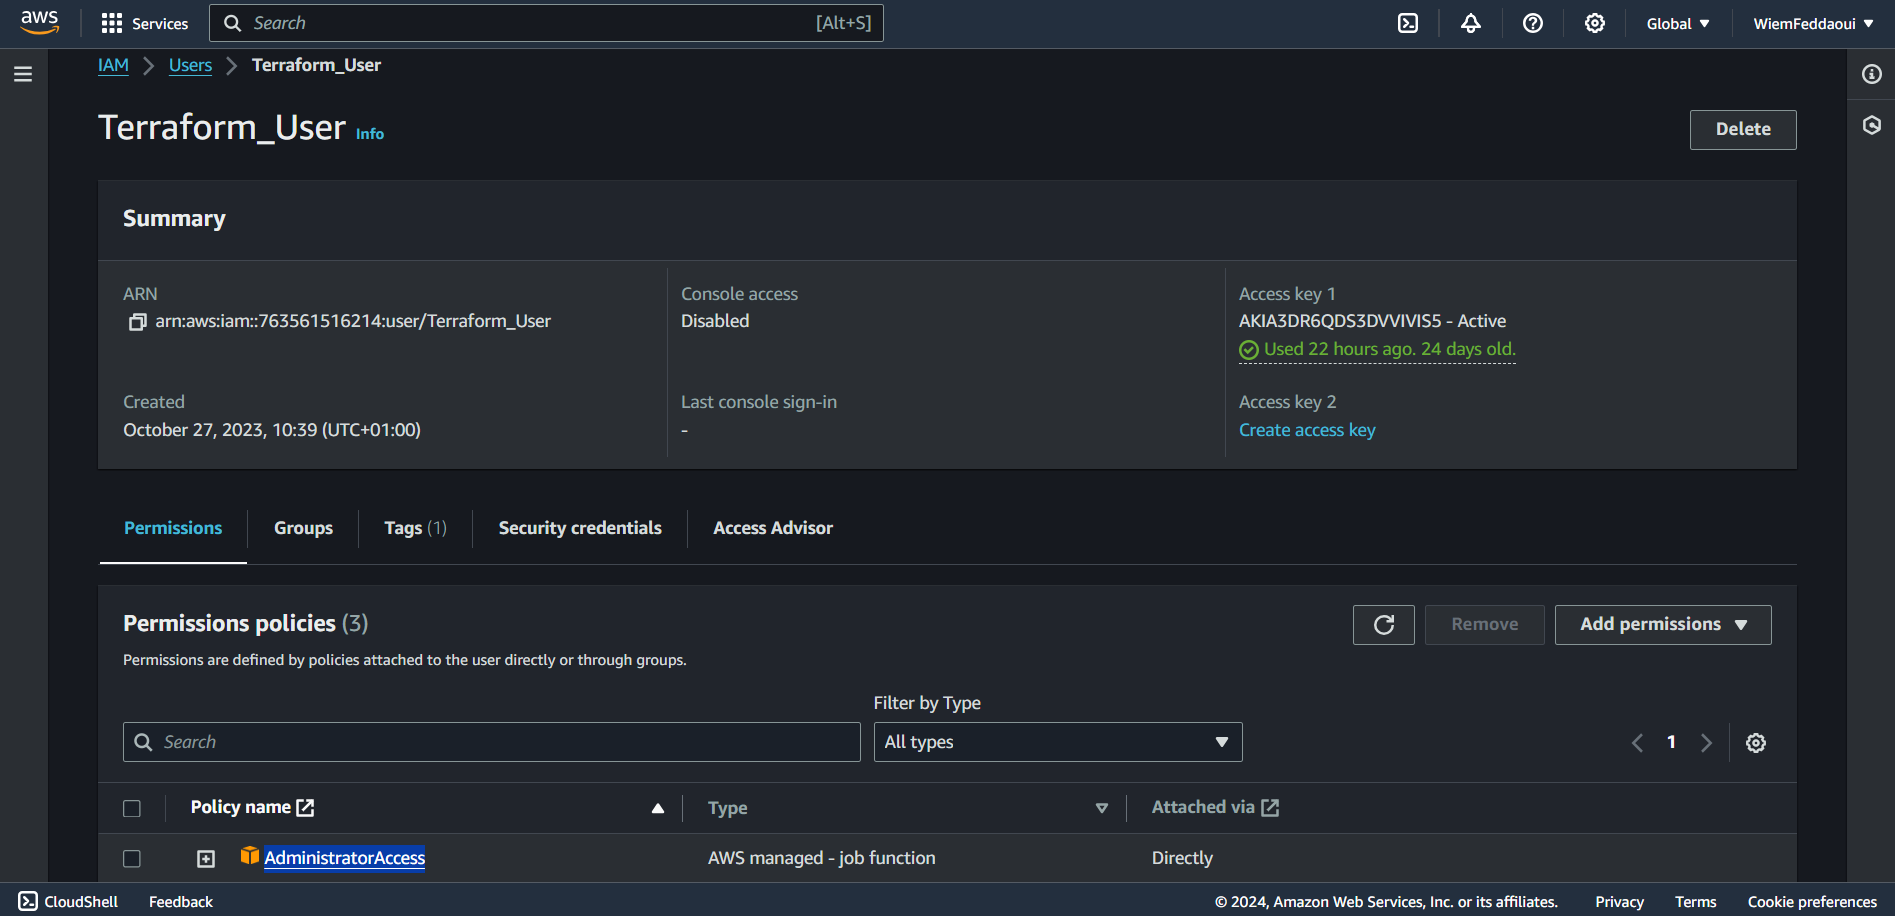
\includegraphics[width=17cm, height=10cm]{img/terraform-user.PNG}}
        \caption{Création d'un utilisateur IAM.}
        \label{fig:terraform_user}
\end{figure}
Cet utilisateur peut avoir des autorisations spécifiques pour contrôler son accès aux ressources AWS, ce qui garantit la sécurité et la gestion des accès aux données et aux services cloud. Dans notre projet, nous attribuons l'accès admin à notre utilisateur IAM.\\ 

La deuxième étape est la création des ressources cloud via Terraform. Nous présentons le code à implémenter afin de créer nos ressources AWS en se basant sur le langage HashiCorp et les coordonnées d'accès de l'utilisateur IAM créé. Ce code est stocké dans le fichier "main.tf". Une partie de ce programme est illustré dans la figure \ref{fig:terraform_main}.
\begin{figure}[H]
        \centering
        \frame{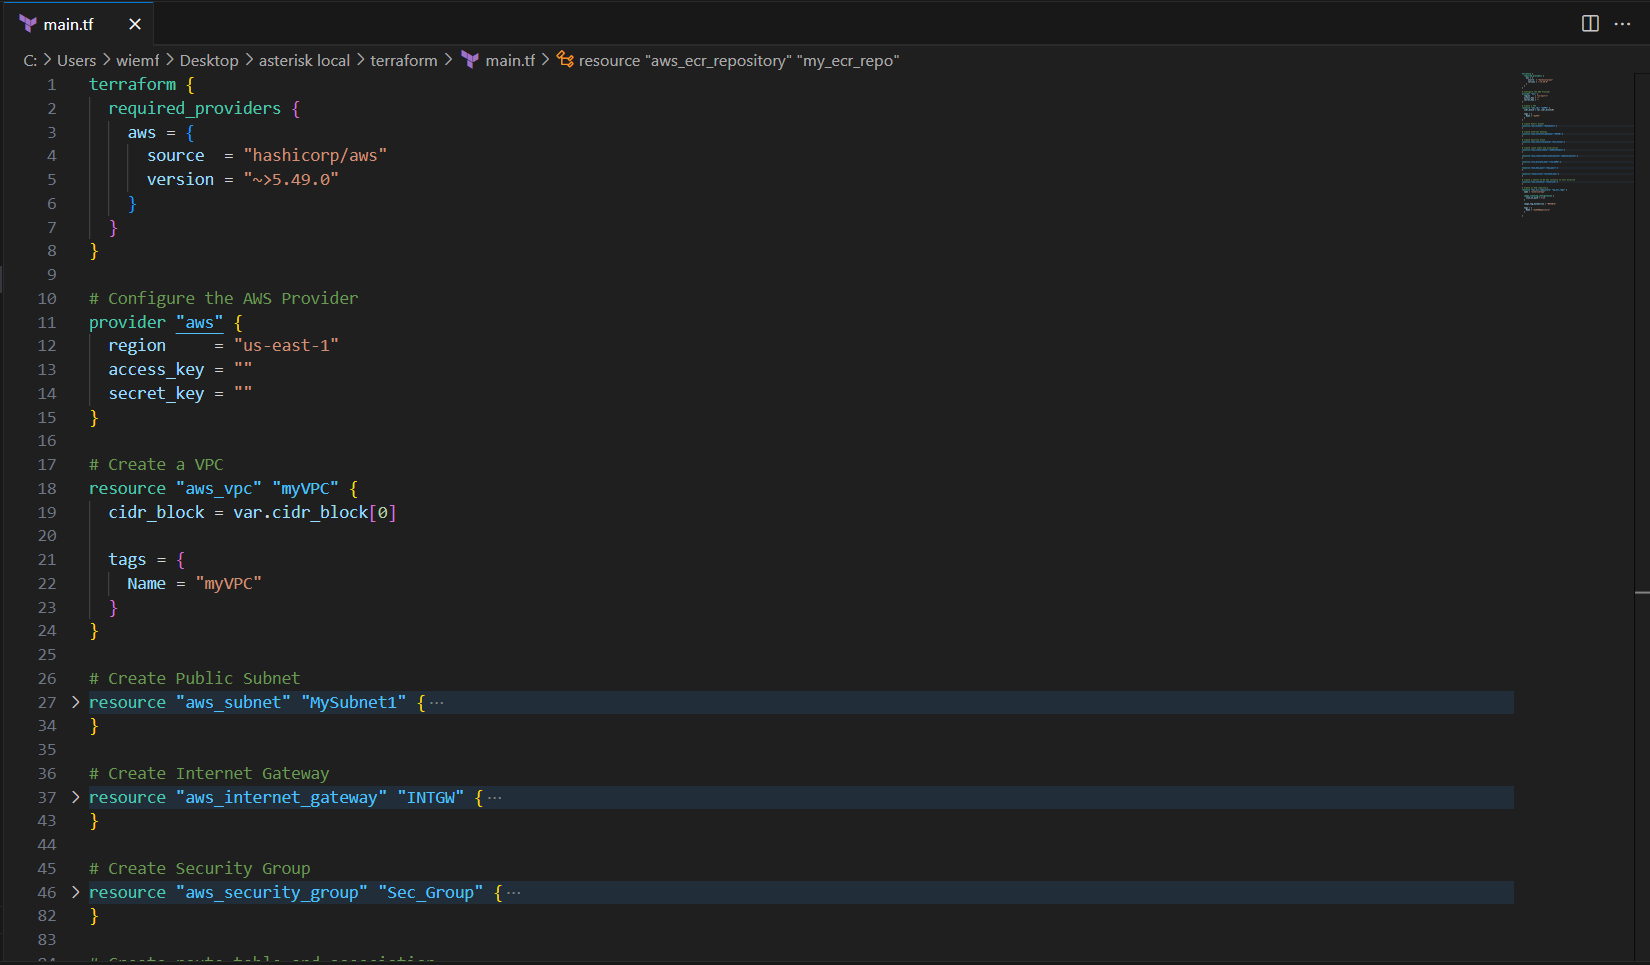
\includegraphics[width=17cm, height=16cm]{img/mainTF.PNG}}
        \caption{Code de création des ressources AWS via Terraform.}
        \label{fig:terraform_main}
\end{figure}
\vspace{2cm}
Nous détaillons alors les ressources à créer :
\begin{itemize}
    \item \textbf{Création d'un VPC:} ce dernier permet de déployer des ressources dans un environnement virtuel isolé, offrant un contrôle total sur leur réseau. Cela inclut la spécification du bloc CIDR définissant l'adresse de ce VPC et l'ajout de tags pour l'identifier.
    \item \textbf{Création d'un Public Subnet:} cette partie décrit la création d'un subnet public dans le VPC précédemment créé. Cette ressource fournit une route vers Internet. Cela signifie que les instances qui se trouvent dans ce subnet peuvent être accessibles depuis Internet.
    \item \textbf{Création d'un Internet Getway:} ici, une passerelle Internet est créée et attachée au VPC. Cette passerelle permet aux ressources du VPC d'accéder à Internet et de recevoir des connexions entrantes depuis le réseau public.
    \item \textbf{Création d'un groupe de sécurité :} cette création définit les règles d'entrée et de sortie du trafic sur des ports spécifiés.
    \item \textbf{Création d'une table de routage et association :} cette partie configure une table de routage pour le VPC, en définissant une route vers l'Internet Getway pour tout le trafic (0.0.0.0/0). Ensuite, la table de routage est associée au subnet public créé précédemment.
    \item \textbf{Génération d'une clé privée :} cette section génère une clé privée RSA de 4096 bits à utiliser pour l'authentification SSH avec l'instance EC2.
    \item \textbf{Création d'une clé public :} une clé publique est créée et elle sera utilisée pour accéder à l'instance EC2.
    \item \textbf{Sauvegarde de la clé privée :} ce bloc de code sauvegarde la clé privée dans un fichier en local. Ce fichier permet l'accès SSH à l'instance EC2.
    \item \textbf{Création d'un dépôt ECR:} ce dépôt créé dans le registre des conteneurs ECR est dédié pour stocker nos images Docker.
    \item \textbf{Création d'une instance EC2 :} cette ressource crée une instance EC2 utilisant l'AMI (Amazon Machine Image) ubuntu 22.04, le type d'instance et la paire de clés générée.\\ L'instance est déployée dans le subnet public, avec une adresse IP publique associée, et elle utilise un script bash d'initialisation pour configurer Docker et Git comme le montre la figure \ref{fig:bash}.
    \begin{figure}[H]
        \centering
        \frame{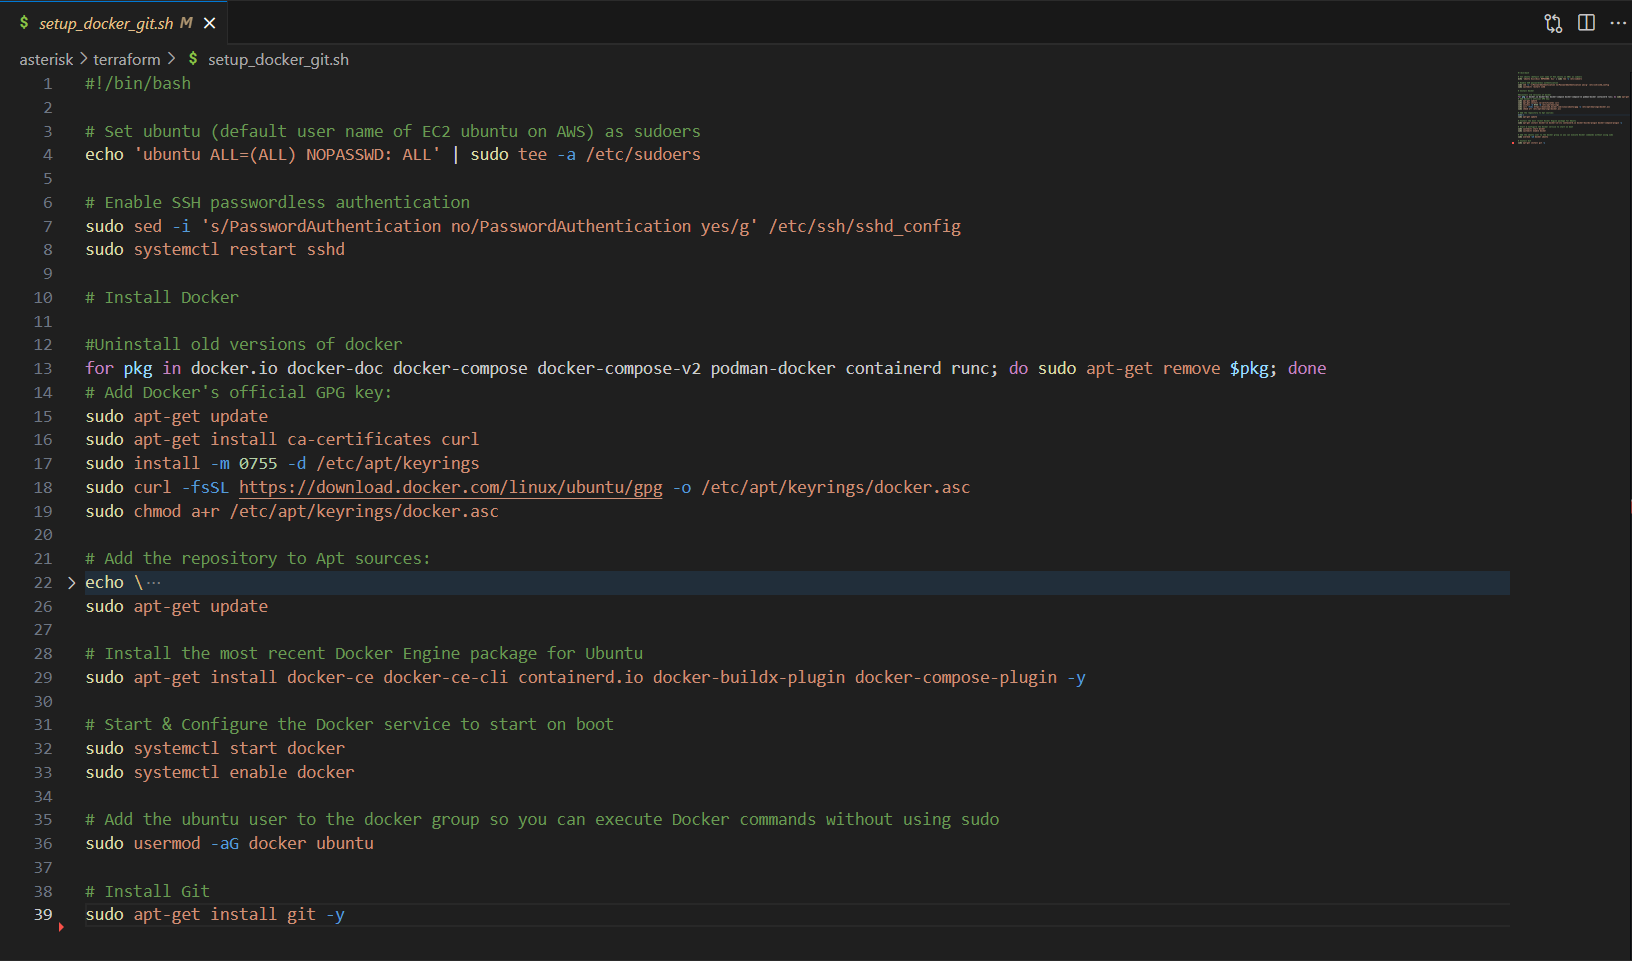
\includegraphics[width=17cm, height=12cm]{img/bash.PNG}}
        \caption{Script bash d'initialisation pour configurer Docker et Git.}
        \label{fig:bash}
    \end{figure}
\end{itemize}

Les variables utilisées dans le fichier "main.tf" sont déclarées dans un fichier "variables.tf", comme le montre la figure \ref{fig:var}.
    \begin{figure}[H]
        \centering
        \frame{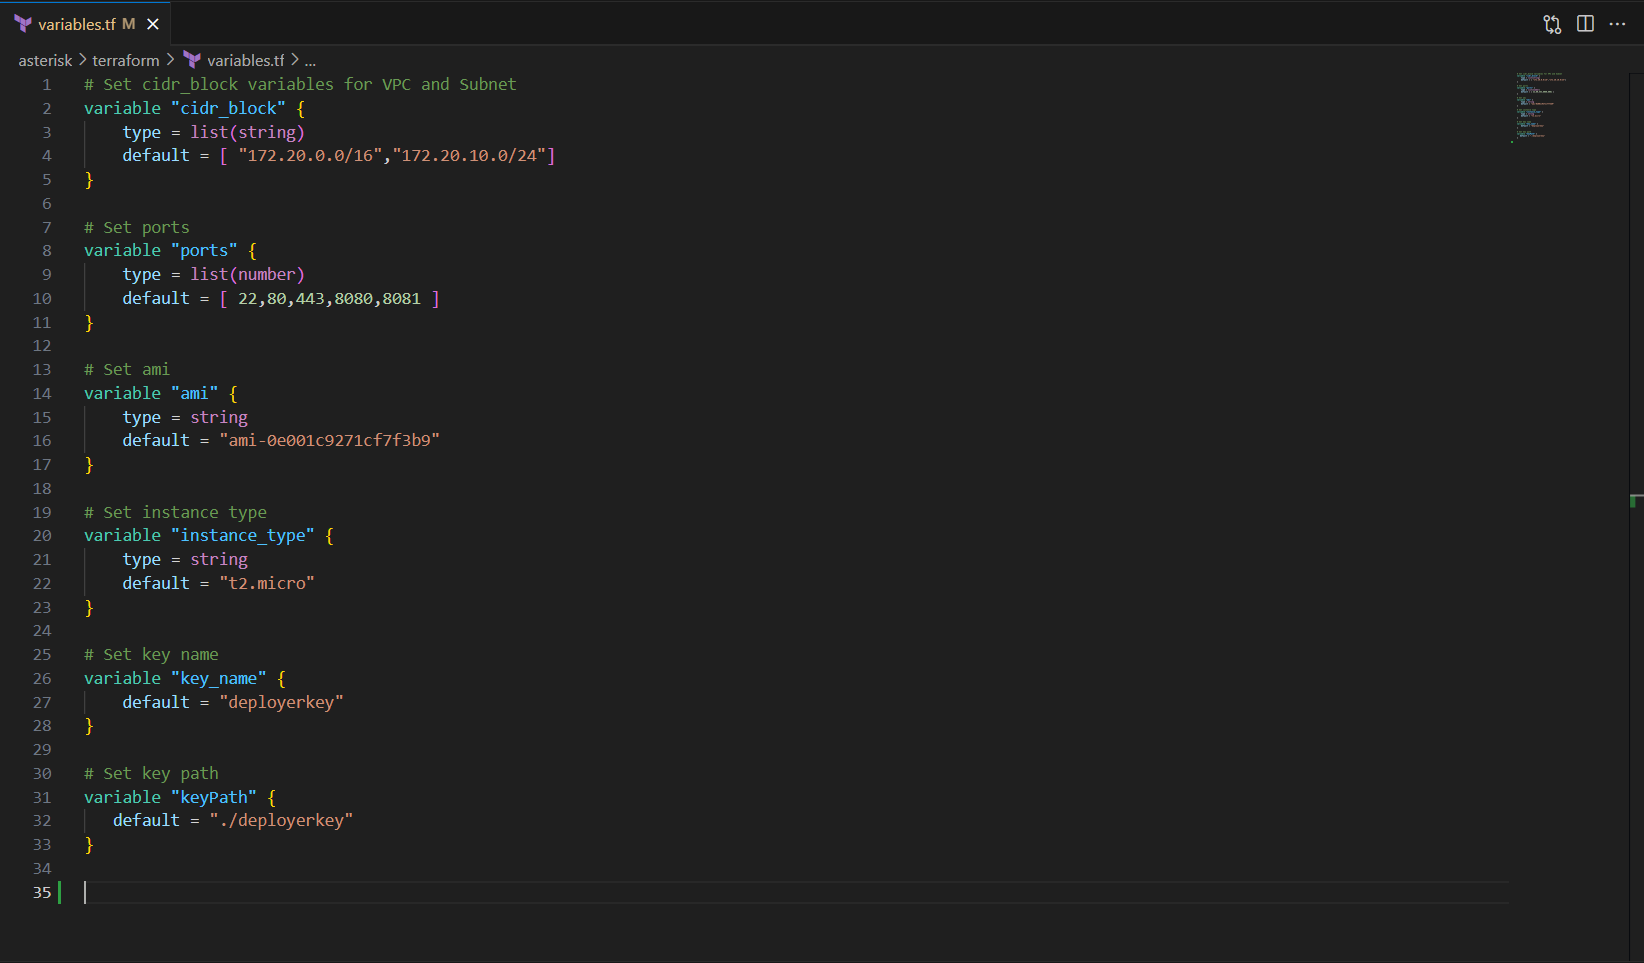
\includegraphics[width=17cm, height=8cm]{img/varTF.PNG}}
        \caption{Code de création des variables Terraform.}
        \label{fig:var}
    \end{figure}

Pour appliquer le code Terraform, nous devons exécuter les trois commandes suivantes :
\begin{itemize}
\item \textbf{Terraform init} pour initialiser le répertoire de travail contenant les fichiers de configuration de Terraform.

\item \textbf{Terraform plan} pour vérifier les modifications qui seront apportées avant de les appliquer.

\item \textbf{Terraform apply} pour appliquer les modifications planifiées.

\end{itemize}

La figure \ref{fig:succes} indique le succès de création de notre infrastructure sur le cloud.
   \begin{figure}[H]
        \centering
        \frame{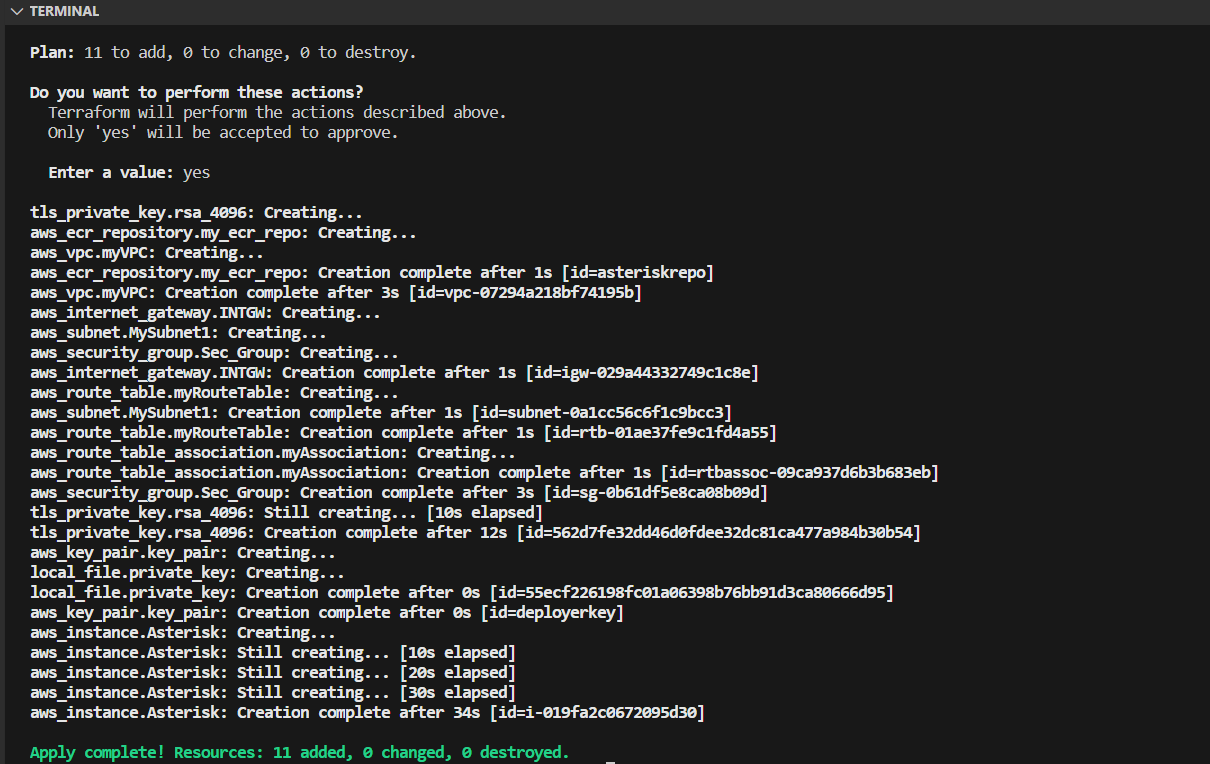
\includegraphics[width=17cm, height=12cm]{img/terminal.PNG}}
        \caption{Succès d'approvisionnement de l'infrastructure.}
        \label{fig:succes}
    \end{figure}

\section{Configuration de serveur Asterisk}
Avant de créer une image Docker pour notre serveur Asterisk, plusieurs fichiers vont être créés et stockées dans /etc/asterisk/. Nous présentons alors ces fichiers et leurs configurations.
\begin{itemize}
    \item \textbf{asterisk.conf:}  ce fichier définit les variables nécessaires à l’utilisation d’Asterisk. Il sert à guider
Asterisk où il doit chercher certains fichiers et les programmes exécutables.\\ La figure \ref{fig:ast} présente le code du fichier.
   \begin{figure}[H]
        \centering
        \frame{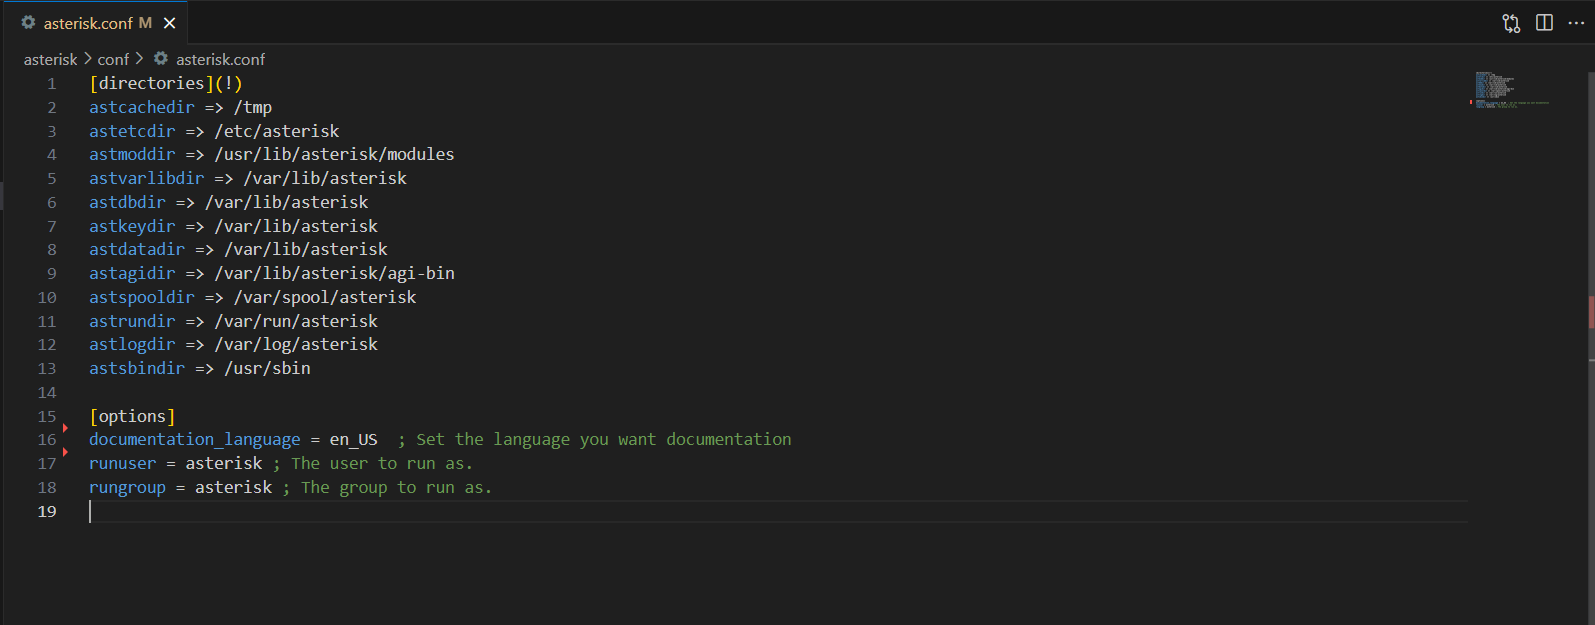
\includegraphics[width=17cm, height=12cm]{img/ast-conf.PNG}}
        \caption{Configuration du fichier "asterisk.conf".}
        \label{fig:ast}
    \end{figure}
    \item \textbf{extconfig.conf:} ce fichier est utilisé pour configurer les sources externes du serveur Asterisk. Il permet d’utiliser des bases de données externes pour stocker des configurations spécifiques. La figure \ref{fig:ext} présente le code du fichier.
   \begin{figure}[H]
        \centering
        \frame{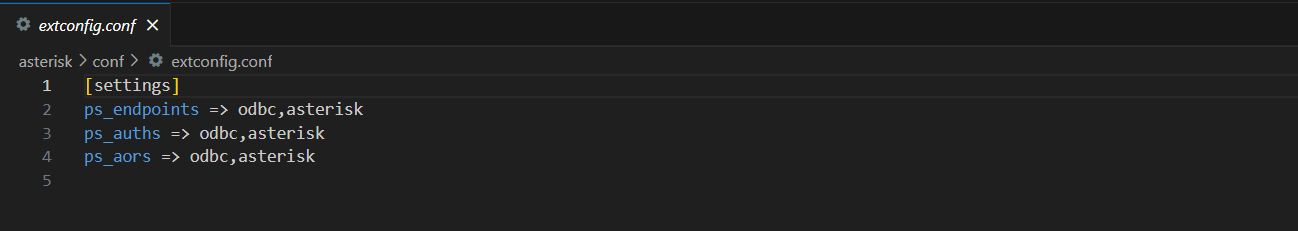
\includegraphics[width=17cm, height=5cm]{img/extconfig.PNG}}
        \caption{Configuration du fichier "extconfig.conf".}
        \label{fig:ext}
    \end{figure}
    \item \textbf{extensions.conf:} ce fichier est utilisé pour définir le plan de numérotation d’Asterisk. Il décrit comment les appels sont traités, dirigés et quelles actions sont effectuées pour chaque numéro composé. La figure \ref{fig:exts} présente le code du fichier.
   \begin{figure}[H]
        \centering
        \frame{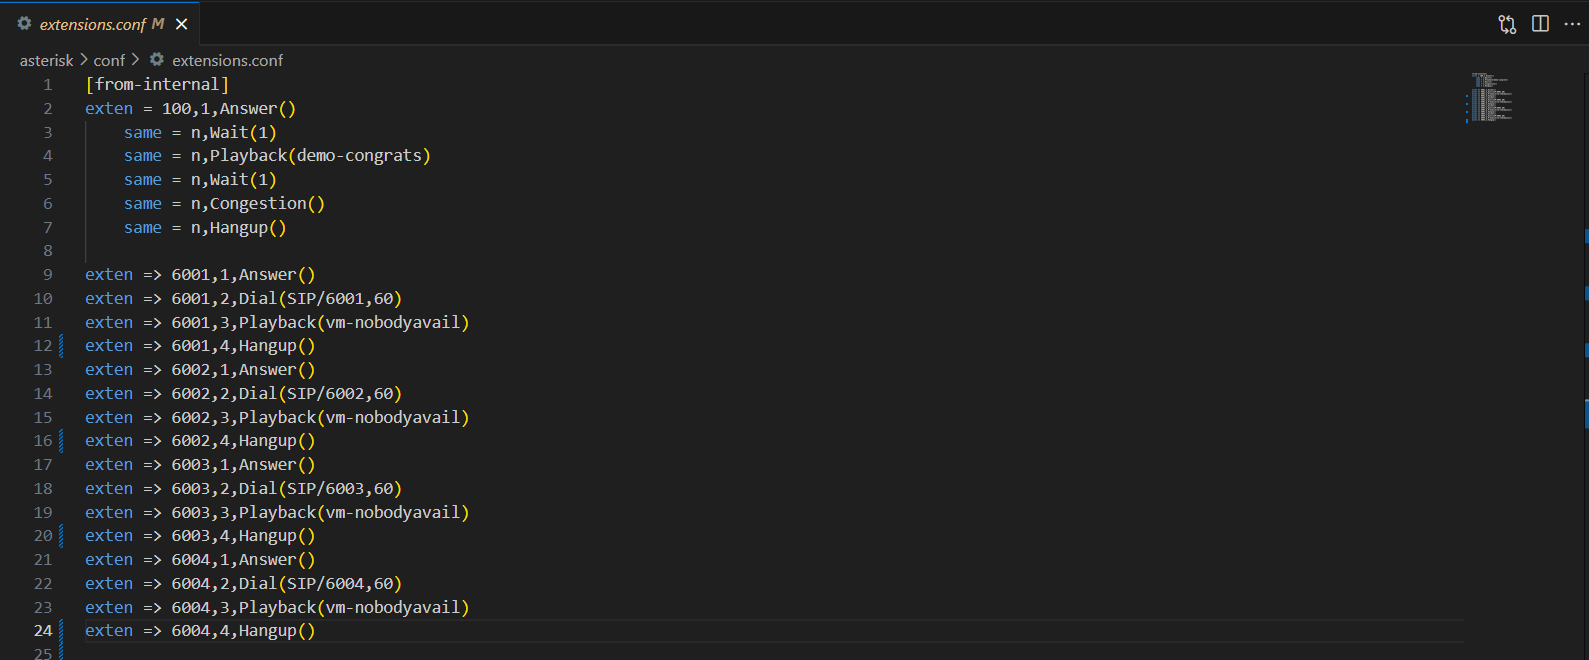
\includegraphics[width=17cm, height=11cm]{img/extensions.PNG}}
        \caption{Configuration du fichier "extensions.conf".}
        \label{fig:exts}
    \end{figure}
    \item \textbf{modules.conf:} ce fichier contrôle quels modules sont chargés ou non au démarrage d’Asterisk. Il permet de gérer les fonctionnalités disponibles dans Asterisk en activant ou désactivant les modules. La figure \ref{fig:mod} présente le code du fichier.
   \begin{figure}[H]
        \centering
        \frame{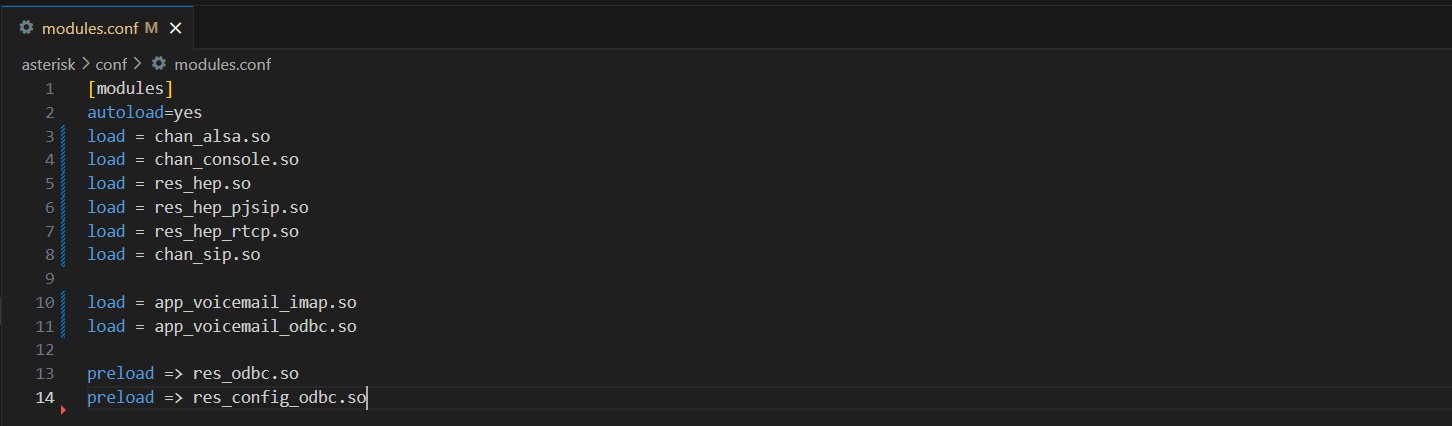
\includegraphics[width=17cm, height=7cm]{img/modules.PNG}}
        \caption{Configuration du fichier "modules.conf".}
        \label{fig:mod}
    \end{figure}
    \item \textbf{pjsip.conf:} ce fichier configure le module PJSIP, utilisé pour la gestion des protocoles SIP dans Asterisk. Il remplace l’ancien sip.conf pour une gestion plus flexible et plus performante des connexions SIP. La figure \ref{fig:pjsip} présente le code du fichier.
   \begin{figure}[H]
        \centering
        \frame{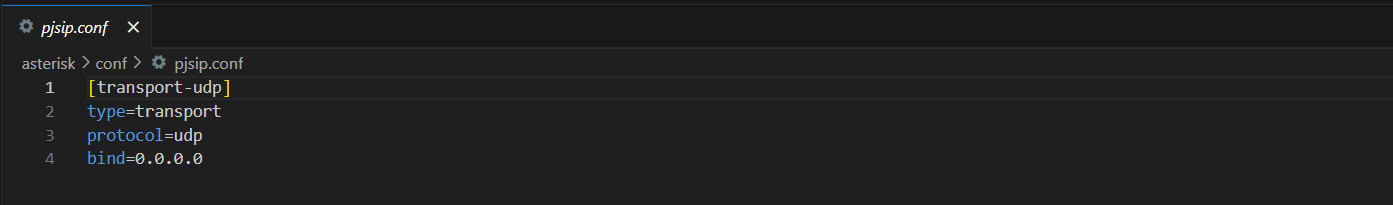
\includegraphics[width=17cm, height=5cm]{img/pjsip.PNG}}
        \caption{Configuration du fichier "pjsip.conf".}
        \label{fig:pjsip}
    \end{figure}
    \item \textbf{res_odbc.conf:} ce fichier configure les connexions ODBC pour Asterisk, permettant à celui-ci de se connecter à des bases de données relationnelles pour des tâches telles que la gestion des CDR (Call Detail Records) et les répertoires de numérotation. La figure \ref{fig:odbc} présente le code du fichier.
   \begin{figure}[H]
        \centering
        \frame{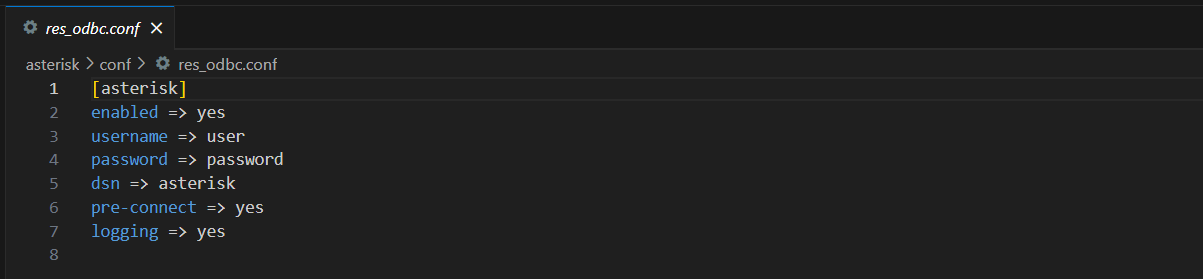
\includegraphics[width=17cm, height=6cm]{img/res_odbc.PNG}}
        \caption{Configuration du fichier "res_odbc.conf".}
        \label{fig:odbc}
    \end{figure}
    \item \textbf{sorcery.conf:} ce fichier configure le système Sorcery d’Asterisk, qui est utilisé pour la gestion des données de configuration en utilisant différents backends de stockage. Il permet de spécifier comment et où les différentes catégories de données de configuration sont stockées et récupérées. La figure \ref{fig:sorcery} présente le code du fichier.
   \begin{figure}[H]
        \centering
        \frame{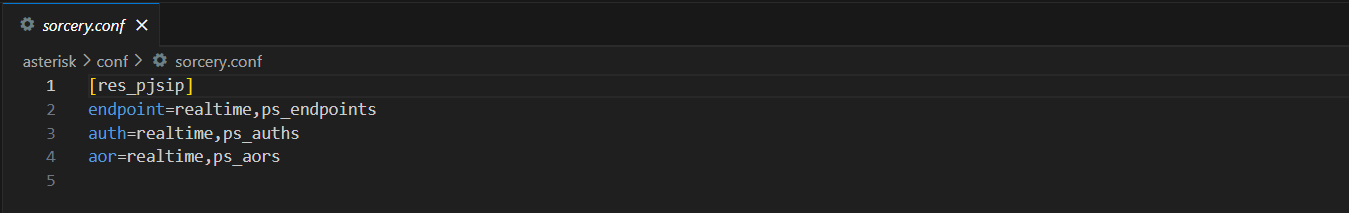
\includegraphics[width=17cm, height=4cm]{img/sorcery.PNG}}
        \caption{Configuration du fichier "sorcery.conf".}
        \label{fig:sorcery}
    \end{figure}
\end{itemize}
Ces fichiers de configuration nous permettent de personnaliser et de contrôler le fonctionnement d’Asterisk. Chacun joue un rôle spécifique dans la gestion des appels, des modules, des protocoles et des connexions aux bases de données, offrant une flexibilité et une extensibilité importante à ce serveur de communication.

\section{Configuration de la base de données MySQL}
Un dump est une sauvegarde de la base de données, souvent utilisée pour restaurer la base de données ou la transférer vers un autre serveur. Dans cette partie, nous créons ce fichier pour définir la structure et les données de certaines tables de la base de données Asterisk. 
\begin{itemize}
    \item La table \texttt{ps\_aors} est définie pour stocker les informations sur les AORs (Address of Records), qui sont des points de contact pour les utilisateurs SIP.
    \item La table \texttt{ps\_auths} contient des informations d'authentification pour les utilisateurs SIP.
    \item La table \texttt{ps\_endpoints} définit les points de terminaison (endpoints) SIP, qui sont les appareils ou logiciels utilisés pour les appels.
\end{itemize}
La figure \ref{fig:dumb} illustre une partie du code de ce fichier.
   \begin{figure}[H]
        \centering
        \frame{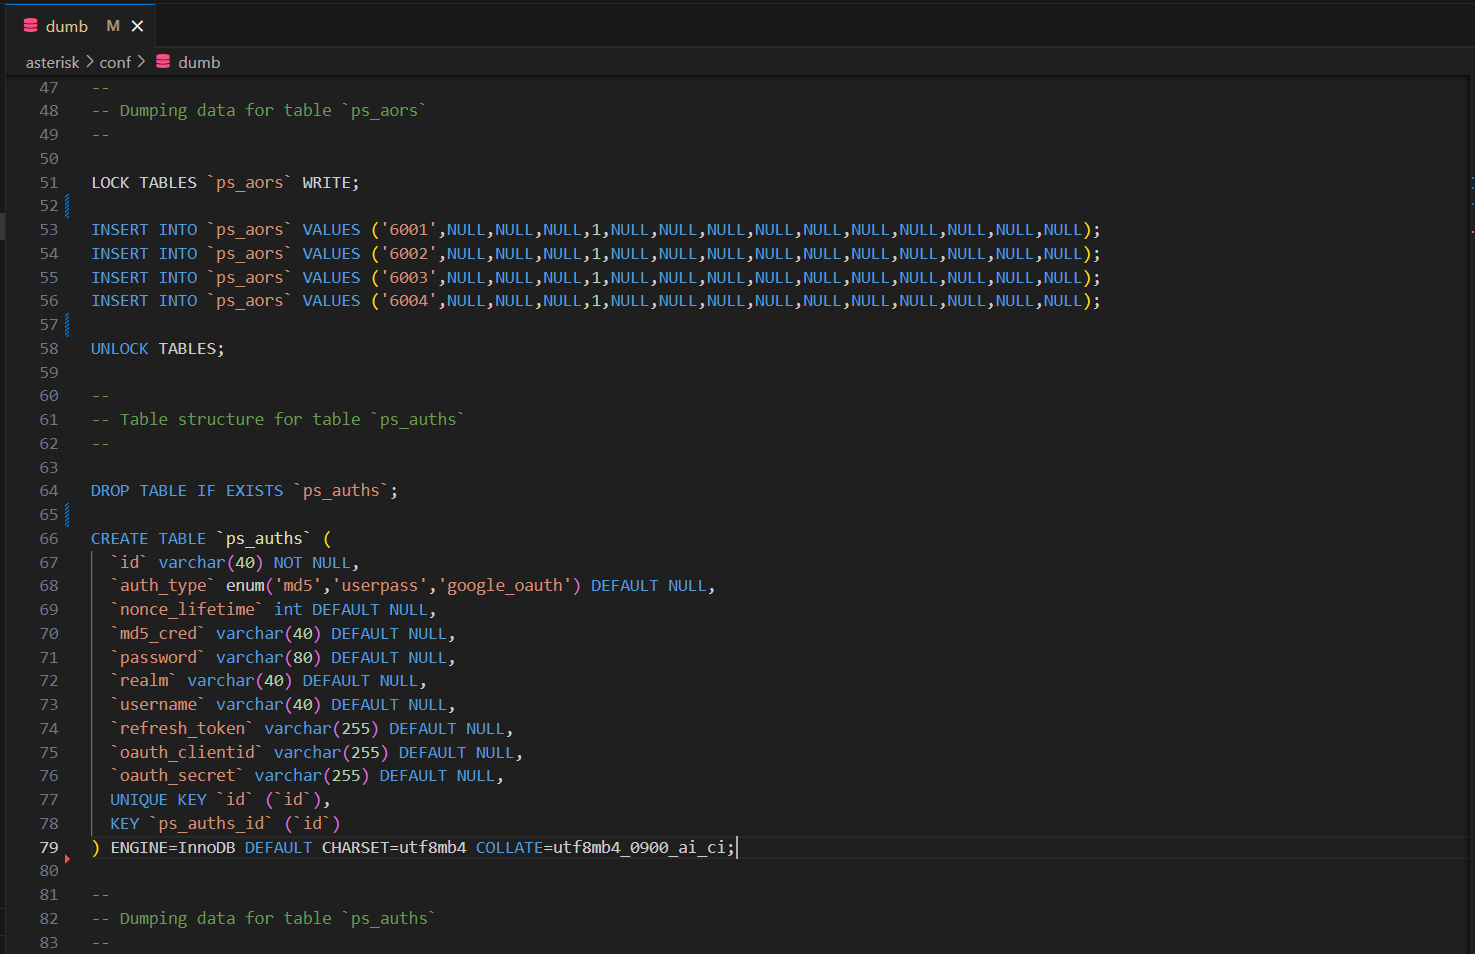
\includegraphics[width=17cm, height=13cm]{img/dumb.PNG}}
        \caption{Configuration du fichier "dumb.sql".}
        \label{fig:dumb}
    \end{figure}

\section{Construction d'une image Docker pour Asterisk} 
La construction d'une image Docker pour le serveur Asterisk implique la création d'un fichier Dockerfile spécifique pour Asterisk, comme illustré dans la figure \ref{fig:dc1}. Ce fichier contient toutes les dépendances, les configurations de port et l'environnement nécessaires pour construire le serveur. L'objectif est de générer une image isolée du reste du code. Cette étape sera intégrée à la première phase de la réalisation du pipeline CI/CD.
\begin{figure}[H]
        \centering
        \frame{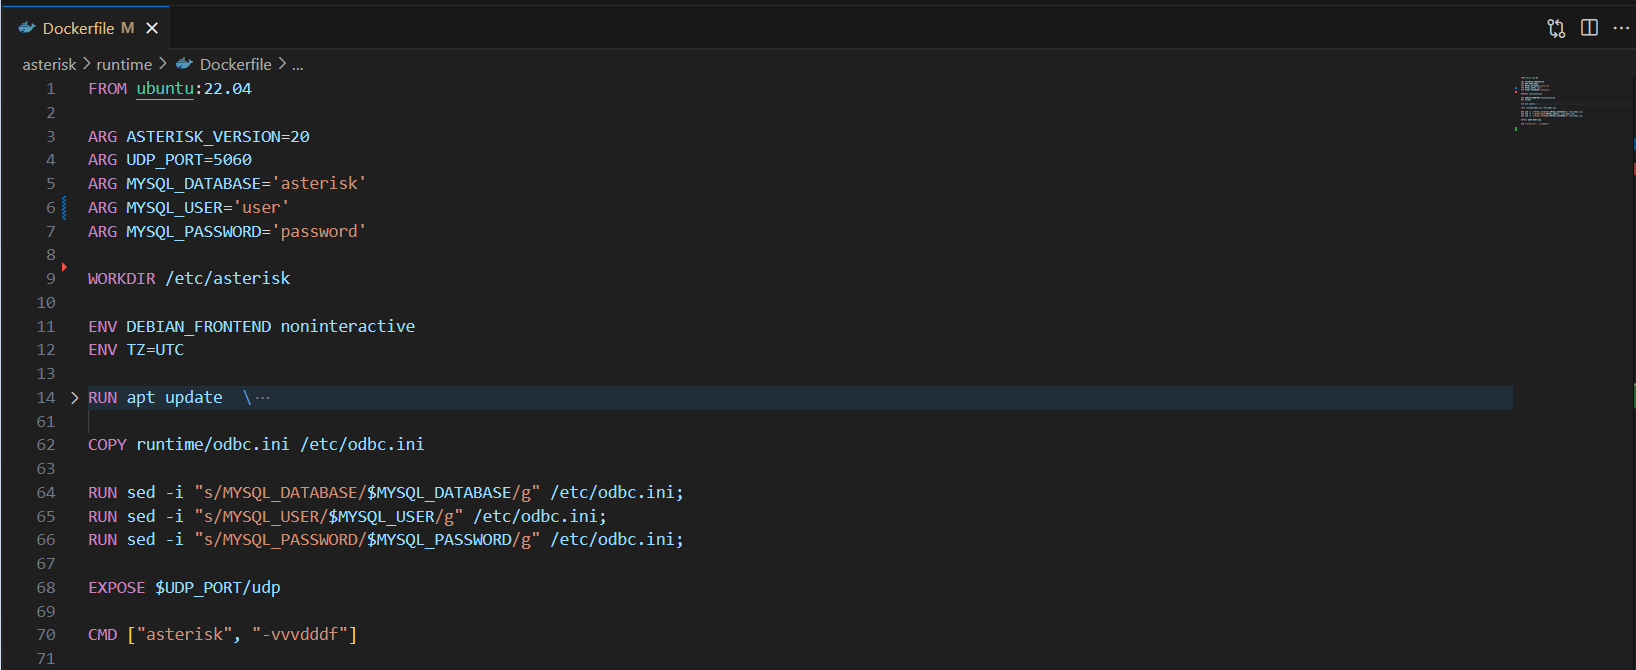
\includegraphics[width=17cm, height=11cm]{img/dockerfile_asterisk.PNG}}
        \caption{Dockerfile du serveur Asterisk.}
        \label{fig:dc1}
        \end{figure}
        
\section{Conteneurisation de l'image Docker Asterisk} 
Cette partie est consacrée à la conteneurisation qui vise à rendre une image Docker exécutable sur n'importe quelle infrastructure.

Pour exécuter l'images Docker créée précédemment, nous utilisons un fichier «docker-compose.yml» présenté dans la figure \ref{fig:dc3}. Ce fichier permet de lancer l'image du serveur Asterisk en parallèle avec l'image de base de données MySQL fournie par Docker. Nous obtenons ainsi deux conteneurs qui sont placés dans le même réseau et peuvent communique ensemble.
\begin{figure}[H]
        \centering
        \frame{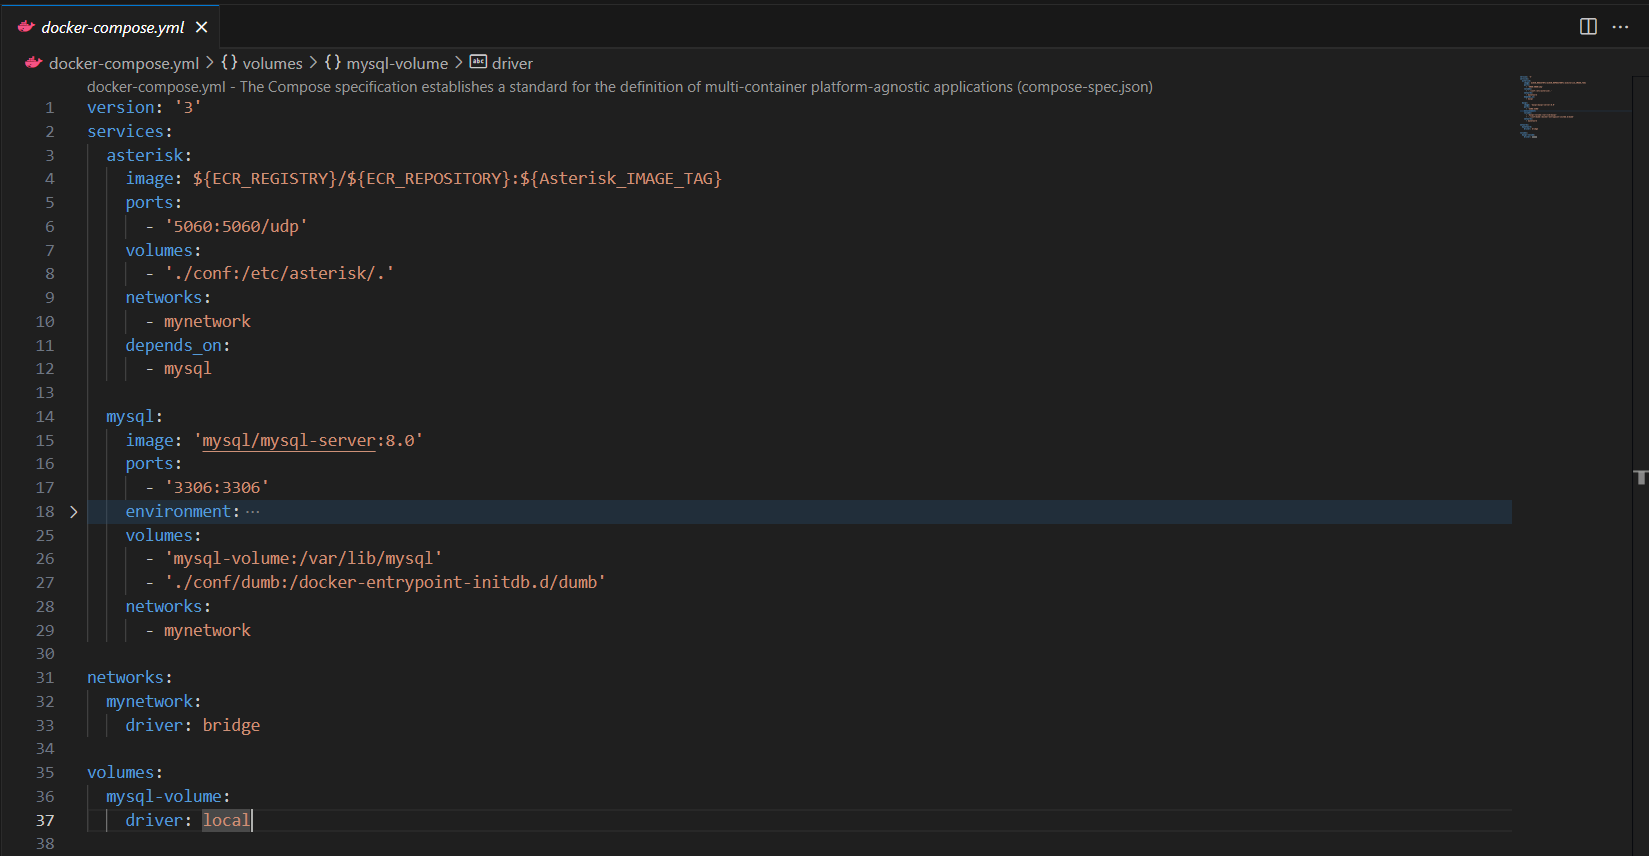
\includegraphics[width=17cm, height=14cm]{img/docker-compose.PNG}}
        \caption{Docker Compose du système Asterisk.}
        \label{fig:dc3}
        \end{figure}

\section{Mise en place d'un pipeline CI/CD}

Après avoir préparé les phases nécessaires pour le pipeline CI/CD d'Asterisk, nous créons le code de ce pipeline et le testons à travers GitHub Actions. Dès qu’un changement est détecté au niveau du code, le pipeline se déclenche automatiquement.
Ce dernier illustré par la figure \ref{fig:cicd}, nommé "Build and Deploy", gère le processus de construction et de déploiement de notre solution utilisant Docker Compose sur une instance EC2.

La section "build" construit et pousse l'image Docker d'Asterisk vers Amazon ECR, tandis que la section "deploy" déploie cette image sur l'instance EC2 spécifiée. Elle supprime également l'ancienne configuration Docker Compose de l'instance, copie les nouveaux fichiers de configuration et les fichiers de configuration d'Asterisk, puis utilise Docker Compose pour démarrer les conteneurs.

En outre, le script de déploiement mentionne la création d'un fichier ".env", qui semble être utilisé pour définir des variables d'environnement nécessaires au déploiement, telles que le registre ECR, le référentiel ECR et le tag de l'image Asterisk. Cependant, il y a une mention d'un fichier "dumb" dans le commentaire final.
\begin{itemize}
    \item Build and Push Asterisk image to ECR : construction et envoi de l’image Docker vers le service ECR d’AWS pour la stocker.
    \item Deploy : l’importation de l’image Docker du serveur Asterisk stockée dans le service ECR et le lancement de Docker Compose sur l’instance EC2 avec un serveur base de données MySQL.
\end{itemize}

\begin{figure}[H]
        \centering
        \frame{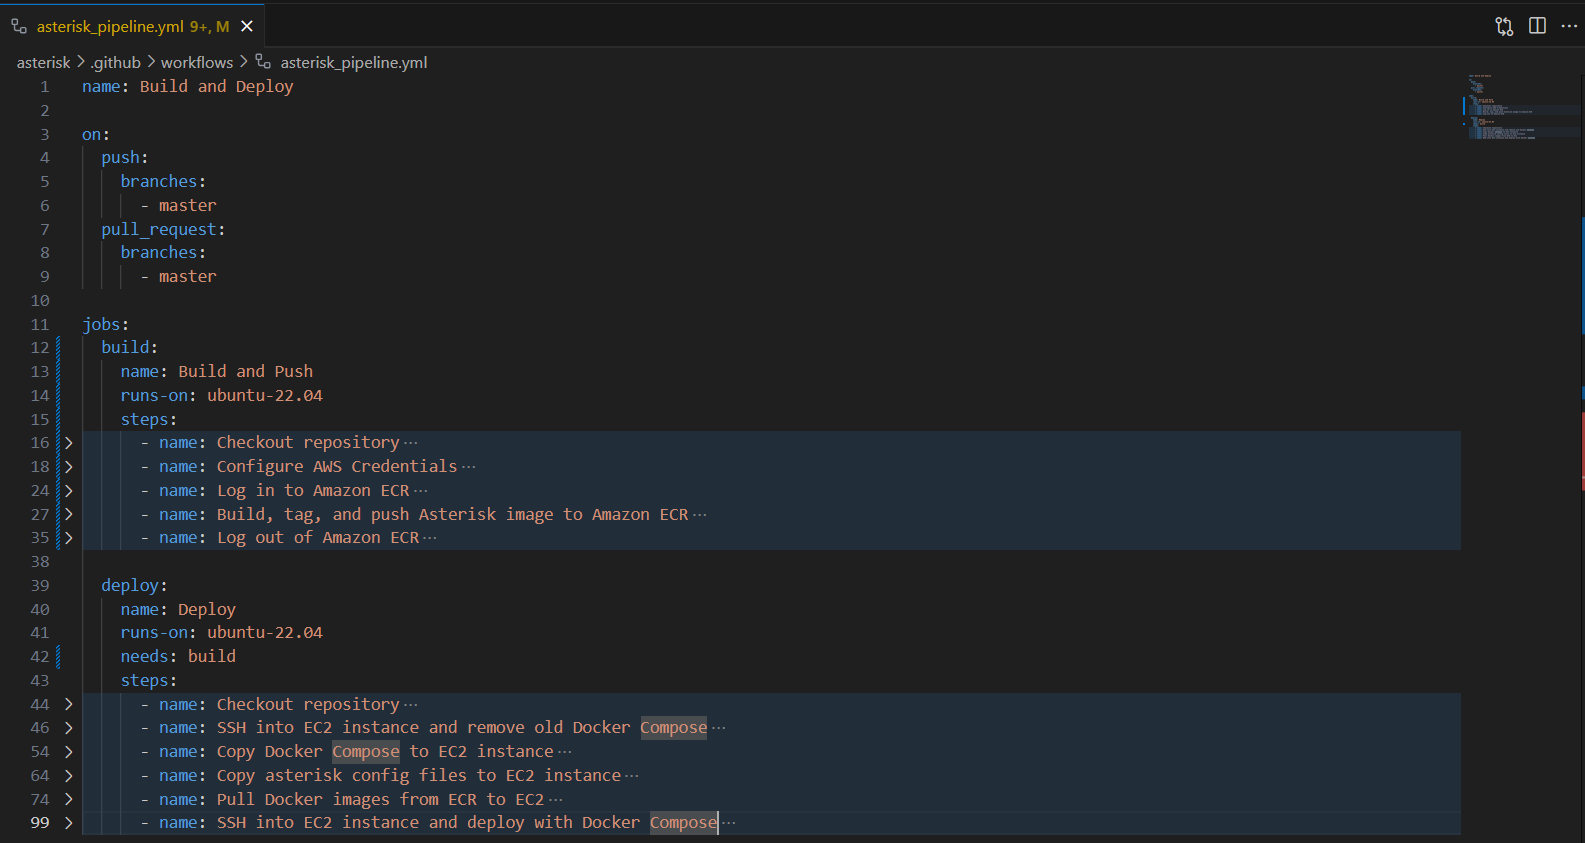
\includegraphics[width=17cm, height=14cm]{img/pipe.PNG}}
        \caption{Pipeline CI/CD du système Asterisk.}
        \label{fig:cicd}
        \end{figure}

La figure \ref{fig:s} présente graphiquement les étapes du pipeline CI/CD du système Asterisk et indique le succès de chaque phase.
\begin{figure}[H]
        \centering
        \frame{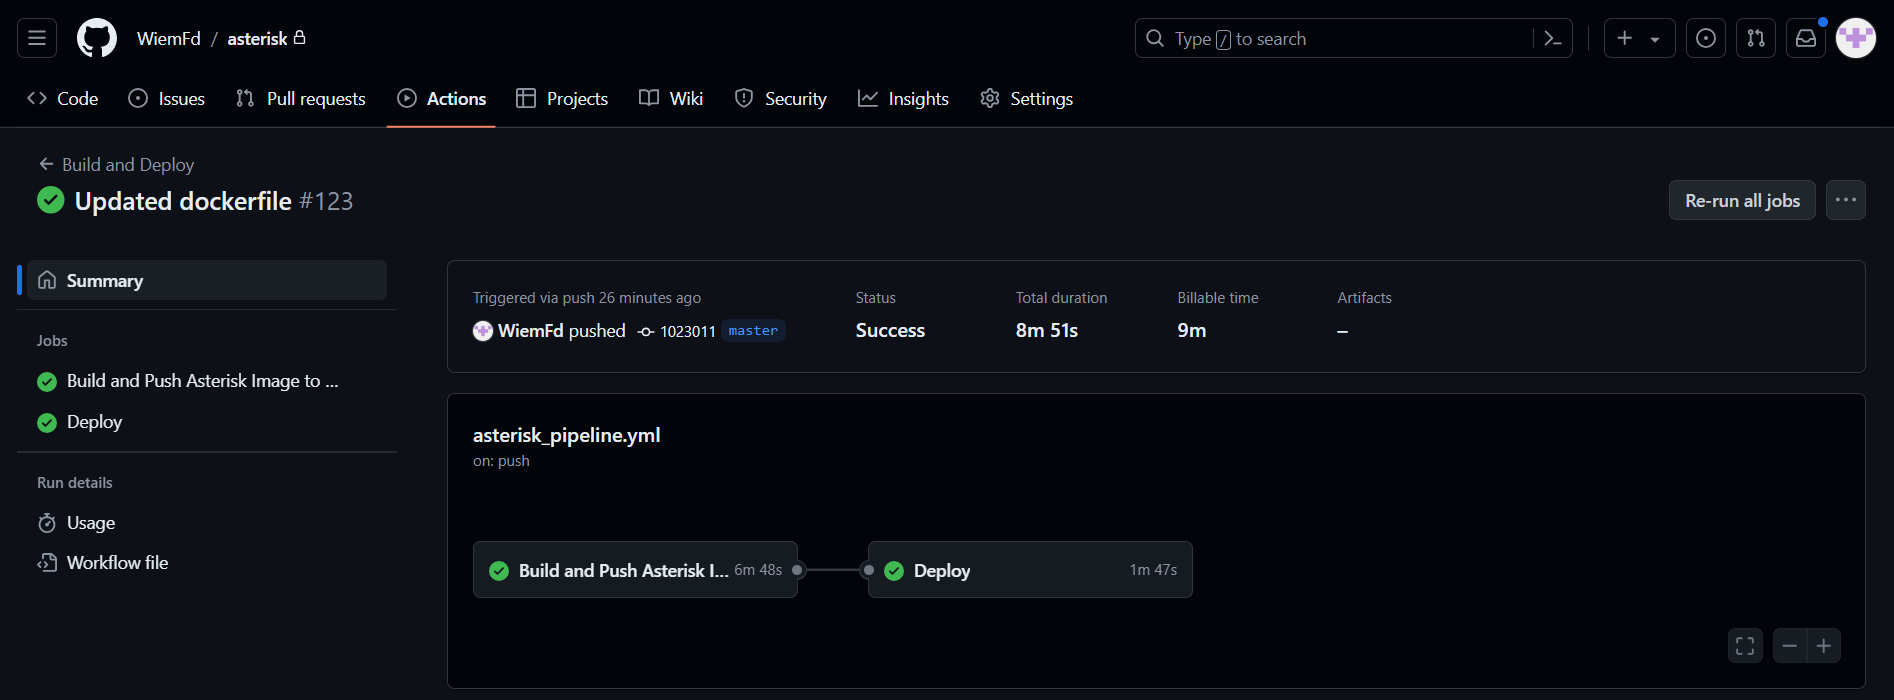
\includegraphics[width=17cm, height=9cm]{img/pipeline_s.PNG}}
        \caption{Représentation graphique de pipeline CI/CD.}
        \label{fig:s}
\end{figure}
Lors de la création du code de pipeline CI/CD, des données sensibles comme les clés d'accès à notre compte AWS, ne doivent pas être affichées en texte clair. Grâce au GitHub Secrets, nous pouvons stockées nos variables de manière cryptée et sécurisé comme le montre la figure \ref{fig:secrets}.
\begin{figure}[H]
        \centering
        \frame{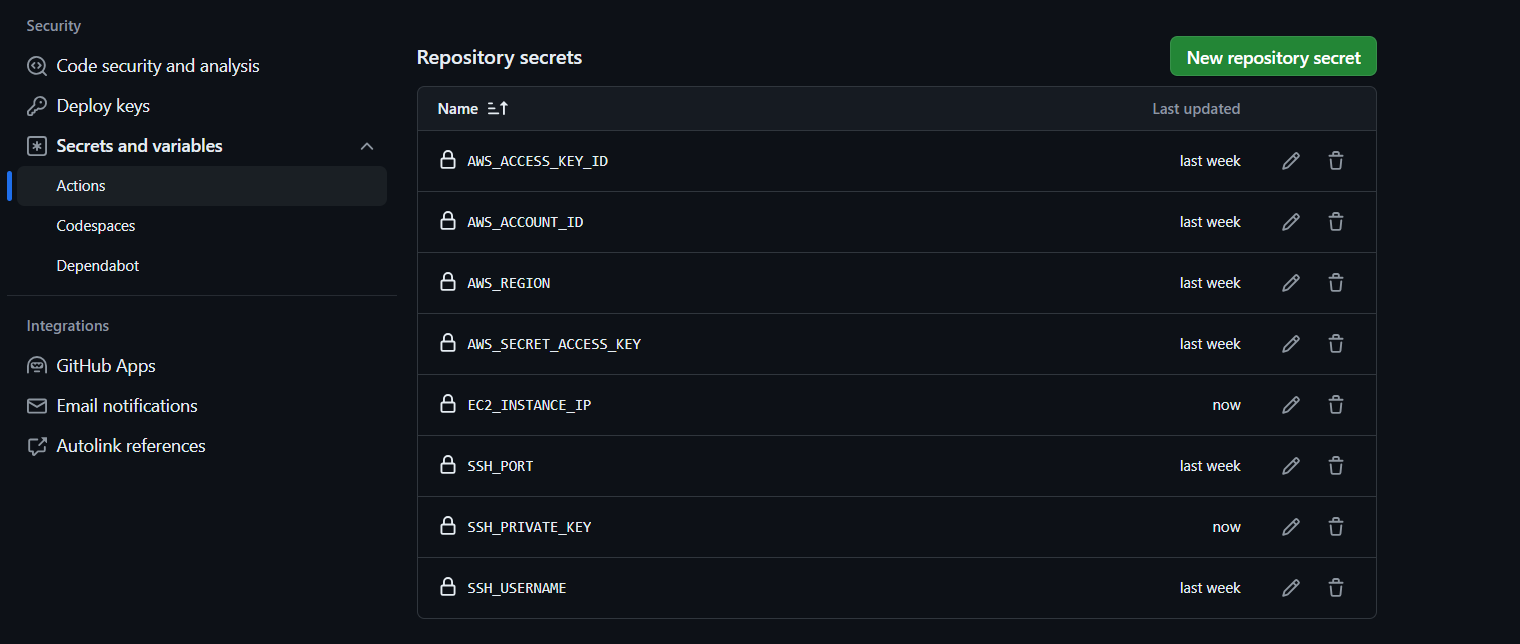
\includegraphics[width=17cm, height=9cm]{img/secrets.PNG}}
        \caption{Stockage des données sensibles sur Github.}
        \label{fig:secrets}
\end{figure}

\section{Test et validation de l'accès au seveur Asterisk}
Dès que le pipeline se termine, les conteneurs Docker seront déployés sur notre instance ubuntu EC2. Pour assurer que ces conteneurs sont créés correctement et en cours d'exécution. Nous devons appliquer la commande "docker ps" présentée dans la figure \ref{fig:ps}.
\begin{figure}[H]
        \centering
        \frame{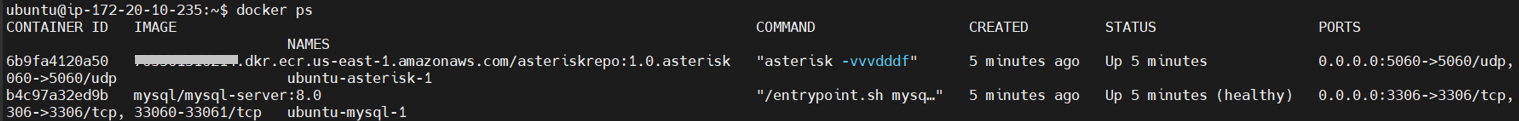
\includegraphics[width=17cm, height=3cm]{img/docker_ps.PNG}}
        \caption{Succès de création des conteneurs Docker.}
        \label{fig:ps}
\end{figure}

Tout d'abord, nous devons établir une connexion SSH avec l'instance AWS via la clé privée copiée en locale lors du processus de l'approvisionnement. Maintenant, nous pouvons accéder à ce conteneur et vérifier le bon fonctionnement de notre service Asterisk en suivant les commandes illustrées dans la figure \ref{fig:ok-asterisk}. 
\begin{figure}[H]
        \centering
        \frame{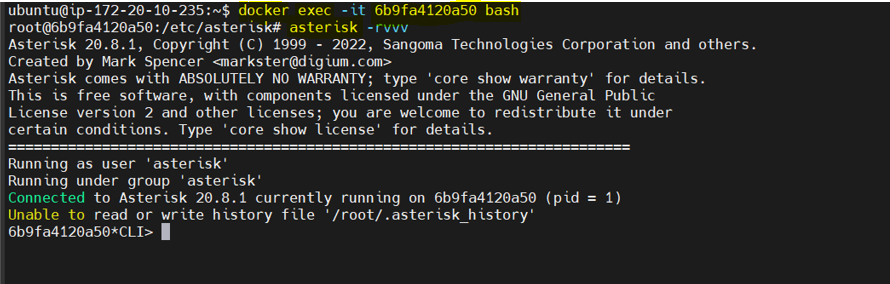
\includegraphics[width=17cm, height=6cm]{img/asterisk-s.PNG}}
        \caption{Succès d'accès au service Asterisk.}
        \label{fig:ok-asterisk}
\end{figure}
Afin de tester un appel audio via Asterisk, nous utilisons l'application client Linphone basée sur le protocole d'initiation SIP.
Cette application possède une version Desktop et une version mobile. Pour se connecter, nous devons utilisés l'adresse publique de notre instance comme domaine SIP, un nom d'utilisateur crée déjà dans notre base de données MySQL ainsi que son mot de passe. Il est important aussi de vérifier si Linphone utilise le port d'accès au serveur Asterisk 5060. Dès que la connexion s'établie, nous tappons 100 pour écouter le message vocale de succès de configuration "demo-congrats".
La figure \ref{fig:ok-linphone} illustre cet appel.
\begin{figure}[H]
        \centering
        \frame{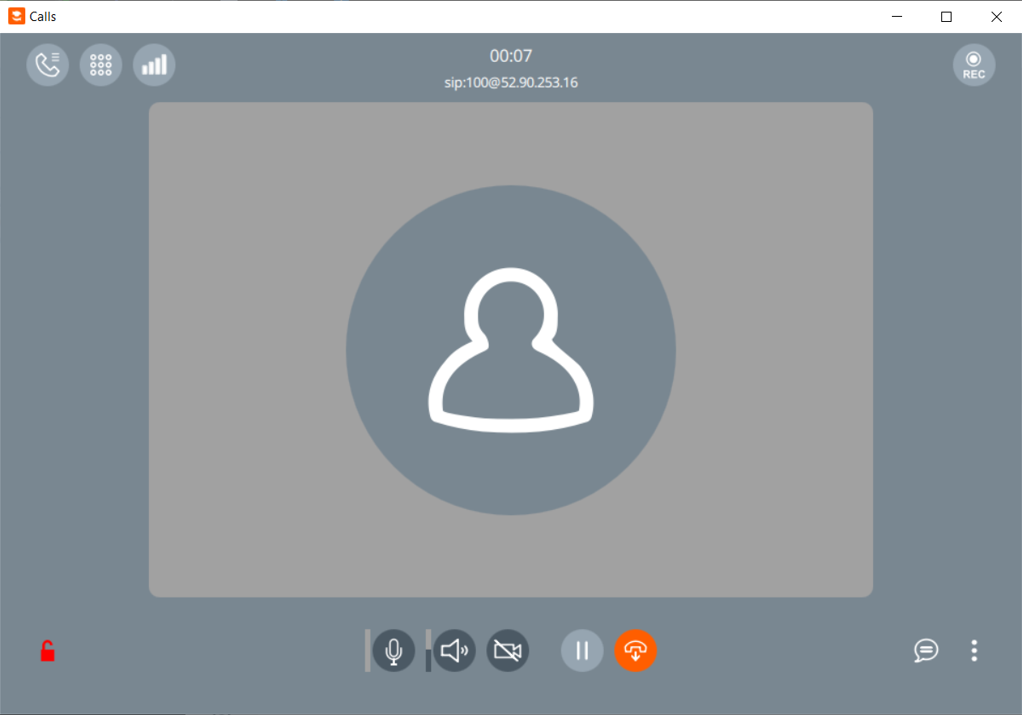
\includegraphics[width=17cm, height=7.25cm]{img/linphone_call.PNG}}
        \caption{Accès au serveur Asterisk à partir de Linphone.}
        \label{fig:ok-linphone}
\end{figure}

\section{Personnalisation de l'application Linphone}
L'application Desktop client Linphone SIP est open-source et développée avec QML/QT5 et C++. Pour commencer à personnaliser cette application, il faut préparer l'environnement de développement et installer les dépendances nécessaires. Le nom est transformé au Bridge et le style de l'application est modifié, comme présenté dans la figure \ref{fig:linphone}.
\begin{figure}[H]
        \centering
      \frame{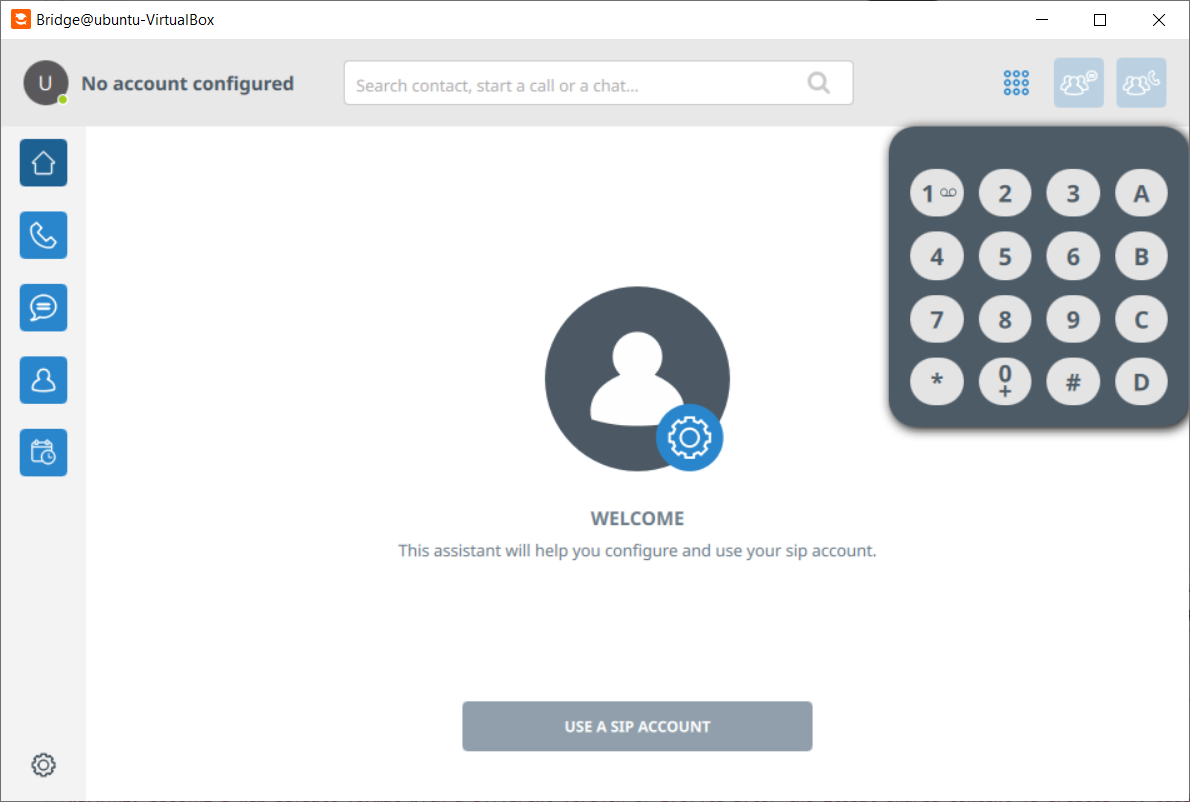
\includegraphics[width=17cm, height=10cm]{img/linphone.PNG}}
        \caption{Application Bridge.}
        \label{fig:linphone}
\end{figure}

\section*{Conclusion}
Ce chapitre nous a permis de présenter, dans un premier temps, la mise en place de la solution en couvrant l'approvisionnement de l'IaC, la création de l'image Docker pour Asterisk, ainsi que la conteneurisation du serveur et la mise en place des phases du pipeline CI/CD. Enfin, nous avons mis en évidence le test et la validation de la connexion au service Asterisk, ainsi que la personnalisation de l'application client Linphone.







